% !TEX root = ../my-thesis.tex
%
\chapter{PROBLEMA A RESOLVER}
\label{sec:problema}

Una vez conocido el estado del arte de la clasificación de malas hierbas y habiendo presentado las bases teóricas del trabajo, se va a pasar a desarrollar en mayor profundidad el problema que motiva este trabajo y la hipótesis de partida para tratar de solucionarlo. Posteriormente, se presentará el conjunto de datos (\textit{datasetç}) seleccionado con el que se comprobará esta hipótesis planteada.

\section{Problema localizado e hipótesis para su resolución}

Como ya se introducía en el estado del arte, en la actualidad, dentro del campo de la agricultura, la agricultura de precisión está tomando bastante protagonismo en los últimos años, debido a las ventajas que supone, económica y medio-ambientalmente. Esto está llevando a crear grandes desarrollos en este área, donde se descubren nuevas barreras tecnológicas que deben ser superadas para la implantación de ciertos sistemas automatizados en el campo.

Uno de estos campos, es la detección y eliminación de malas hierbas, ya ya que estas compiten con la cosecha por los recursos que aportar el campo, lo que limita de gran manera la producción total, por lo que en la actualidad, se trata de realizar trabajos de eliminación de estas plagas de forma extensiva. Esto no es una forma adecuada de aplicarse, debido a que podría afectar al desarrollo del cultivo, además de que se emplean grandes cantidades de correctivos que no son realmente necesarios.

La solución que se propone por tanto, es la localización y clasificación de forma precisa de estas malas hierbas en los cultivos de forma automatizada, aplicando correctivos de forma puntual a estas de forma selectiva y eficaz a cada una de ellas. Para esto, se ha trabajado en los últimos años en desarrollos donde se trata de emplear las últimas técnicas de clasificación de imágenes para abordar las dificultades y problemáticas de la clasificación de diferentes tipos de plantas.

Una de estas técnicas, cada vez está más estandarizada, es el uso de redes neuronales convolucionales, las cuales son entrenadas con un conjunto de datos de muestra etiquetadas, siendo capaces de extraer propiedades visuales de cada uno de los tipos de plantas para posteriormente clasificarlas de forma correcta. Para esto, se emplean redes como las presentadas en el capítulo anterior, las cuáles son arquitecturas genéricas capaces de clasificar de forma eficiente gran número de tipos de imágenes, empleando grandes conjuntos de datos con los que son entrenadas,  que conlleva grandes tiempos de entrenamiento asociados y amplia capacidad computacional de lo cual, no siempre se dispone. Para ello, se propone la solución de usar estas redes pre-entrenadas, de manera que inicialmente ya son capaces de clasificar una elevada cantidad de tipos de imágenes, por lo que luego solo es necesario re-entrenarlas con el \textit{dataset} objetivo, con menores tiempos de entrenamiento \cite{Olsen2019}.

Esta técnica trae varias problemáticas consigo. Una de ellas es que estas redes, para poder tener la capacidad de clasificar numerosos tipos de imágenes, tienen que tener tamaños excesivamente grandes, tanto en número de capas como de parámetros, y la tendencia en los últimos años es que sigan creciendo. En la Tabla \ref{tab:tamaño_cnn}, se pueden ver algunos ejemplos de los tamaños de estas redes.

\begin{table}[h]
\caption{Tamaño de algunas de las CNNs más empleadas en los últimos años}
\label{tab:tamaño_cnn}
\centering
\begin{tabular}{l|r|r}
\toprule
\multicolumn{1}{c|}{\textbf{Red Neuronal Convolucional}} & \multicolumn{1}{c|}{\textbf{Número de capas}} & \multicolumn{1}{c}{\textbf{Parámetros}} \\ \hline
LeNet \cite{lesnet}                                                    & 5                                             & $60 \cdot 10^3$                                   \\
AlexNet \cite{NIPS2012_c399862d}                                                 & 8                                             & $62 \cdot 10^6$                                \\
VGG-16 \cite{simonyan2015deep}                                                   & 16                                            & $138 \cdot 10^6$                               \\
Inception V1 \cite{szegedy2014going}                                            & 22                                            &  $7 \cdot 10^6$                                 \\
Inception V3 \cite{szegedy2015rethinking}                                             & 159                                           & $23 \cdot 10^6$                                \\
Resnet-50 \cite{He2016}                                               & 50                                            & $25 \cdot 10^6$         \\
\bottomrule
\end{tabular}
\end{table}

Lo anterior puede ser válido si estas redes van a ser ejecutadas en equipos con gran potencia computacional, pero es una gran limitación si se quieren emplear en \textit{edge devices}, los cuáles no cuentan con una amplia potencia computacional capaz de mover grandes redes en tiempo adecuados. Además cuenta con otra desventaja, que es el gran número de datos que son necesarios para entrenar estas redes tan ``genéricas''. Además, al tener tamaños más grandes, estas redes son más complicadas de analizar y conocer su comportamiento real, debido al gran número de parámetros que entran en el juego de estas.

Para esto, se pretende buscar una manera de obtener CNNs de menor tamaño, más especializadas, más rápidas e igual de eficientes a la hora de clasificar un \textit{dataset} dado. Para ello, se cree que una opción adecuada de optimizar la arquitectura de estas redes es empleando algoritmos de optimización como son los Algoritmos Evolutivos, más específicamente, los Algoritmos Genéticos. Estos tienen gran un rendimiento a la hora de optimizar grandes problemas que con otros algoritmos ha sido complicado llegar a una solución válida, por lo que se intuye que pueden ser de gran ayuda para la resolución del problema anteriormente comentado.

Como se puede observar, este es un trabajo que puede servir en numerosos campos donde la clasificación de imágenes es un punto crítico y que debe ser optimizado. Aún así, este trabajo en particular se centrará específicamente en el la clasificación de diferentes tipos de malas hierbas.

Por tanto, en este trabajo se tratará de verificar si la hipótesis realizada es cierta y si empleando Algoritmos Genéticos para el diseño de nuevas arquitecturas de CNNs, las realizan de manera que sean más pequeñas, más especializadas y más rápidas manteniendo un desempeño similar al que se obtiene con las soluciones actuales.

\section{Datos a clasificar}

Para alcanzar el objetivo de este trabajo, se debe tener una base de datos suficientemente grande y con cierta calidad, para poder comprobar el desempeño de las arquitecturas extraídas. Es por ello que se seleccionó el \textit{dataset} publicado para el desarrollo de aplicaciones de clasificación de diferentes clases de malas hierbas nativas en Australia \cite{Olsen2019}.

Este \textit{dataset}, cuenta con un total de 17509 imágenes clasificadas, donde se recogen un total de 8 especies diferentes de malas hierbas y un conjunto separado de plantas que no son malas hierbas, denominados negativos. Estas han sido recopiladas de diferentes lugares de Australia como se puede observar en la Figura \ref{fig:loc_malas_hierbas}. Estas especies seleccionadas están localizadas más específicamente en las siguientes zonas de pastoreo a lo largo del estado de Queesland: ``Black River'', ``Charters Towers'', ``Cluden'', ``Douglas'', ``Hervey Range'', ``Kelso'', ``McKinlay'' y ``Paluma''.

Este \textit{datset} incluye imágenes etiquetadas de las siguientes especies: ``Chinee apple'', ``Snake weed'', ``Lantana'', ``Prickly acacia'', `` Siam weed'', ``Parthenium'', ``Rubber vine'' y ``Parkinsonia''. Una recopilación de algunas de las imágenes de cada especie puede verse en la figura \ref{fig:dataset_ejemplo_grande}.

Esta amplia recopilación de imágenes permitirá distinguir entre diferentes tipos de malas hierbas, además de diferenciarlas de aquellas que no lo son, de manera que se podrá comprobar el rendimiento de las arquitecturas obtenidas con el desarrollo del algoritmo planteado durante este trabajo.

\begin{figure}[h]
    \centering
    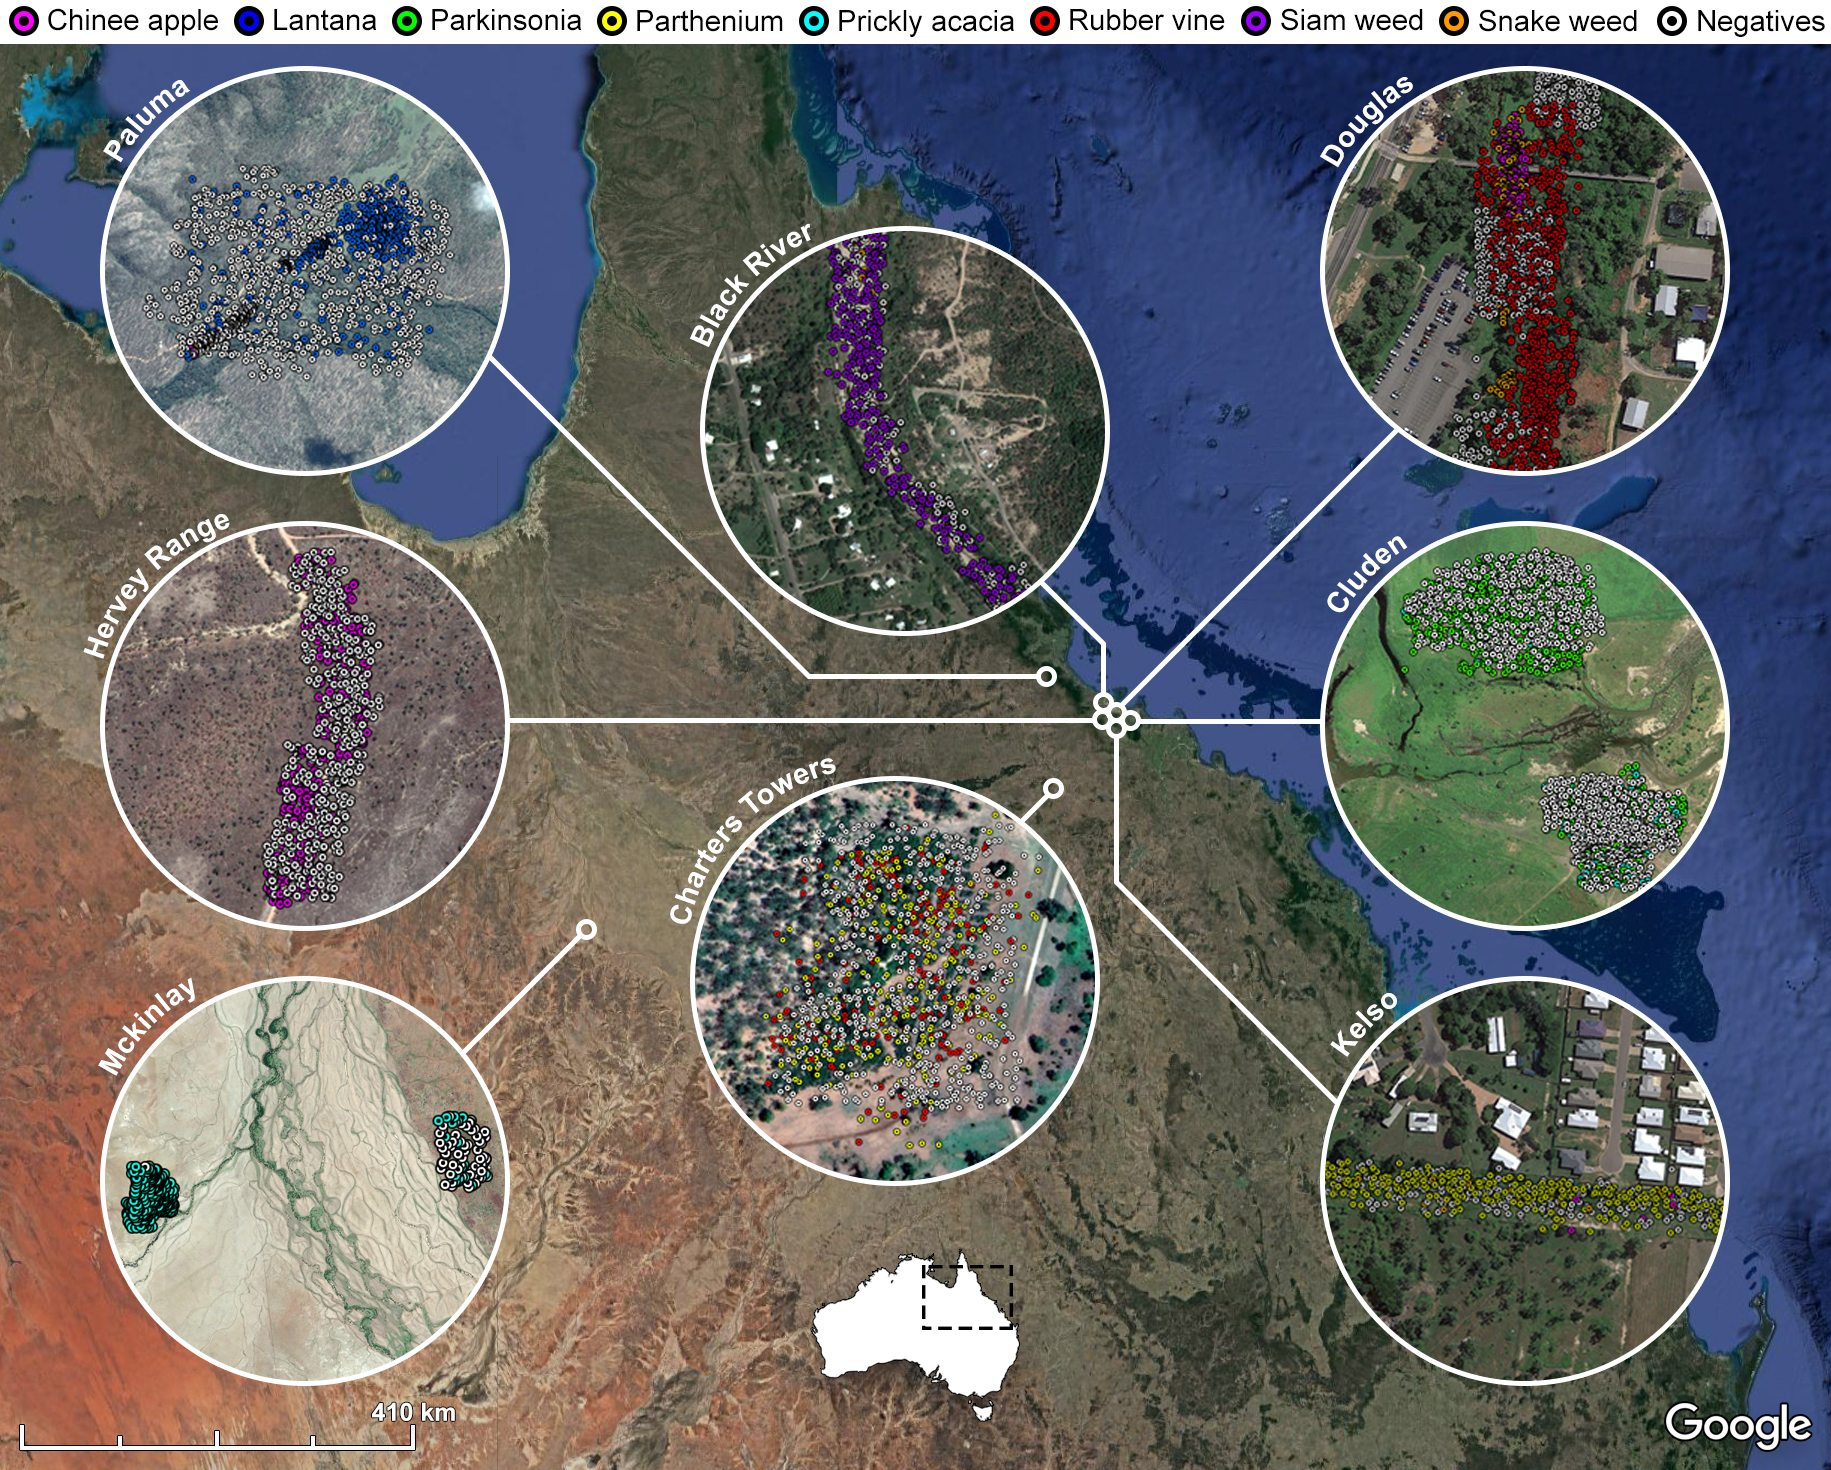
\includegraphics[width=0.95\textwidth]{figuras/problema/localizacion_malas_hierbas.jpg}
    \caption{Localización de las imágenes etiquetadas de malas hierbas del \textit{dataset} seleccionado \cite{Olsen2019}}
    \label{fig:loc_malas_hierbas}
\end{figure}

\begin{figure}[!h]
\centering
    \begin{subfigure}{0.24\textwidth}
        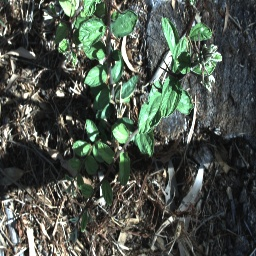
\includegraphics[width=\textwidth]{figuras/problema/chinee_apple.jpg}
        \caption{Chinee Apple}
    \end{subfigure}
    \hfill
    \begin{subfigure}{0.24\textwidth}
        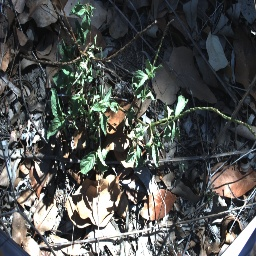
\includegraphics[width=\textwidth]{figuras/problema/snake_weed.jpg}
        \caption{Snake Weed}
    \end{subfigure}
    \hfill
    \begin{subfigure}{0.24\textwidth}
        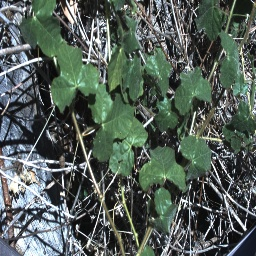
\includegraphics[width=\textwidth]{figuras/problema/lantana.jpg}
        \caption{Lantana}
    \end{subfigure}
    \hfill
    \begin{subfigure}{0.24\textwidth}
        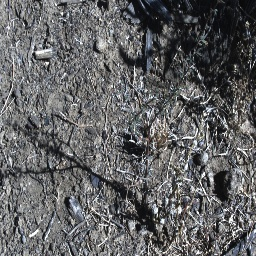
\includegraphics[width=\textwidth]{figuras/problema/prickly_acacia.jpg}
        \caption{Prickly Acacia}
    \end{subfigure}
    \hfill
    \begin{subfigure}{0.24\textwidth}
        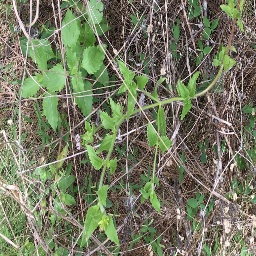
\includegraphics[width=\textwidth]{figuras/problema/siam_weed.jpg}
        \caption{Siam Weed}
    \end{subfigure}
    \hfill
    \begin{subfigure}{0.24\textwidth}
        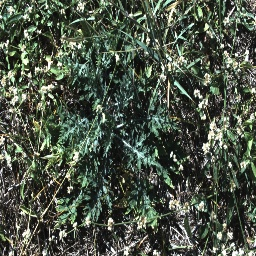
\includegraphics[width=\textwidth]{figuras/problema/parthenium.jpg}
        \caption{Parthenium}
    \end{subfigure}
    \hfill
    \begin{subfigure}{0.24\textwidth}
        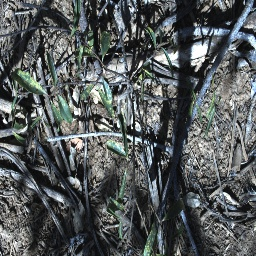
\includegraphics[width=\textwidth]{figuras/problema/rubber_vine.jpg}
        \caption{Rubber Vine}
    \end{subfigure}
    \hfill
    \begin{subfigure}{0.24\textwidth}
        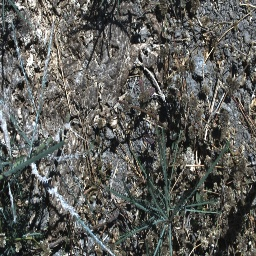
\includegraphics[width=\textwidth]{figuras/problema/parkinsonia.jpg}
        \caption{Parkinsonia}
    \end{subfigure}
    \caption{Imágenes de las diferentes especies recogidas en el \textit{dataset}}
    \label{fig:dataset_ejemplo_grande}
\end{figure}

